\documentclass[a4paper,12pt]{article}
\usepackage[english]{babel}
\usepackage[margin=1in]{geometry}
\usepackage{setspace}
\usepackage{xr} %cross references

% These are used in the preable (which is by Birgitta Burger)
\usepackage{tabularx}
\usepackage{hhline}

\usepackage[most]{tcolorbox} %for scaling
\usepackage{graphicx} %for resizing table
\usepackage{rotating} %for rotating table
\usepackage{hyperref} %for links

\usepackage[backend=bibtex, style=chicago-authordate]{biblatex}

\graphicspath{ {/home/heidi/Gradu2_0/Images/} }
\addbibresource{mastersthesis.bib}

\usepackage[utf8]{inputenc} %whenever Islandic names
\usepackage[T1]{fontenc}

\defbibfilter{literature}{
	type=article or
	type=book or
	type=inbook
}

\title{Game of Networks: Family Ties Within the Swedish Council of the Realm (1523-1680)}
\begin{document}
	\pagenumbering{roman}
	% This front matter is from Birgitta Burger's tex template (v 1.1)
%
\begin{titlepage}
    \mbox{}\vfill
    \begin{center}
        {\bf\Large Game of Networks: Family Ties Within the Swedish Council of the Realm (1523-1680)}\\
        \vfill
        \begin{flushright}
            Heidi Suurkaulio\\[4pt]
            Master's thesis\\[4pt]%change this to term paper or whatever you like
            Historia, yleinen / history, general\\[4pt]
            Historian ja etnologian laitos / Department of History and Ethnology\\[4pt]
            \today\\[4pt]
            Jyväskylän yliopisto / University of Jyväskylä
        \end{flushright}
    \end{center}
\end{titlepage}

\thispagestyle{empty}

{\bf\Large JYVÄSKYLÄN YLIOPISTO}

{\renewcommand{\arraystretch}{1.5}%local redefining of cell spacings
\begin{tabularx}{\textwidth}{|| X | X ||}
\hhline{|t:==:t|}
Tiedekunta -- Faculty		\newline		Humanistis-yhteiskuntatieteellinen tiedekunta	
&
Laitos -- Department		\newline		Historian ja etnologian laitos
\\\hhline{||--||}

\multicolumn{2}{|| p{\textwidth} ||}{
Tekijä -- Author 			\newline		Heidi Suurkaulio
}\\\hhline{||--||}

\multicolumn{2}{|| p{\textwidth} ||}{
Työn nimi -- Title 			\newline		Game of Networks: Family Ties Within the Swedish Council of the Realm (1523-1680)
}\\\hhline{||--||}

Oppiaine -- Subject			\newline 		Historia, yleinen
&
Ty\"on laji -- Level 		\newline		Pro gradu -tutkielma
\\\hhline{||--||}	

Aika -- Month and year		\newline		toukokuu 2025
&
Sivum\"a\"ar\"a -- Number of pages	\newline		47
\\\hhline{||--||}

\multicolumn{2}{|| p{\textwidth} ||}{
Tiivistelmä -- Abstract		\newline
Pro gradu -työni aiheena on Ruotsin valtaneuvosten väliset sukuverkostot aikavälillä 1523-1680. Työni yhdistää digitaalisia ihmistieteitä ja esimodernin ajan tutkimusta. Työn teoreettinen viitekehys ja menetlemä on tietokoneavusteinen verkostoanalyysi.
\newline
Työn aineistona on käytetty Marko Hakasen ja Ulla Koskisen kokoamaa \textit{Swedish Councillors of the Realm, 1523-1680} -tietokantaa. Aineistoon tallennetut valtaneuvosten sukulaisuussuhteet erotellaan automaattisesti omaksi tietorakenteekseen toteuttamallani Python-ohjelmalla. Varsinainen verkostoanalyysi, eli verkon visuaalinen esitys ja tunnuslukujen lasku, on tehty Gephi-työkalulla. Tämän lisäksi aineistosta lasketaan analyysia tukevia (tilastollisia) tunnuslukuja R-ohjelmointiympäristössä.
\newline
Kysymyksenasettelu työssäni liittyy sekä aineistoon että menetelmään. Verkostoanalyysi vahvistaa aikaisemman tutkimuksen antamaa kuvaa siitä, että Ruotsin ylhäisaateli oli varhaismodernilla ajalla verkostoitunutta niin suorien perimyssuhteiden kuin avioliittojenkin kautta. Erityisesti 1600-luvun verkosto on aikaisempaa 1500-luvun verkostoa tiheämpi. Valtaneuvosten verkostoista löytyi kuitenkin myös yksittäisiä henkilöitä, joilla ei ollut takanaan virallista sukuverkostoa. Sosiaalinen ja kansainvälinen liikkuvuus oli siis mahdollista, vaikkakin harvinaista.
\newline
Parhaimmillaan tietokoneavusteinen verkostoanalyysi tuottaa ennalta-arvaamatonta tietoa aineiston rakenteesta, ja tiedon käsittelyn automatisointi ohjelmoimalla nopeuttaa tutkimusprosessia sekä vähentää ihmisen tekemiä (kirjoitus)virheitä. Aineiston käsittelyn automatisointi vaatii kuitenkin aineiston tuntemusta ja tarkkuutta, eivätkä kaikki verkostoanalyysissä käytetyt tunnusluvut sellaisenaan sovi historiallisen sosiaalisen verkoston analysointiin.
}\\\hhline{||--||}

\multicolumn{2}{|| p{\textwidth} ||}{
Asiasanat -- Keywords		\newline
verkostoanalyysi, digihumanismi, varhaismoderni aika, Ruotsin valtakunta, valtaneuvosto, Gephi, Python, R, network analysis, computational history, early modern period, Swedish council of the Realm, Riksrådet
}\\\hhline{||--||}

\multicolumn{2}{|| p{\textwidth} ||}{
Säilytyspaikka -- Depository \newline
Jyväskylän yliopiston kirjasto
}\\\hhline{||--||}

\multicolumn{2}{|| p{\textwidth} ||}{
Muita tietoja -- Additional information
\newline
Git-sivusto: \url{https://github.com/Heidi-Suurkaulio/mastersthesis/} 
}\\\hhline{|b:==:b|}
\end{tabularx}
}
	\newpage
	\maketitle
	\tableofcontents
	\listoftables
	\listoffigures
	\begin{onehalfspace}
		\newpage
		\pagenumbering{arabic}
		\documentclass[a4paper,12pt]{article}
\usepackage[english]{babel}
\usepackage[margin=1in]{geometry}
\usepackage{setspace}
\usepackage{graphicx} %for table
\usepackage[backend=bibtex, style=chicago-authordate]{biblatex}
\addbibresource{mastersthesis.bib}
%whenever Islandic names
\usepackage[utf8]{inputenc}
\usepackage[T1]{fontenc}

\begin{document}
\begin{onehalfspace} %TODO move to the main tex component!
\section{Introduction}
The aim of my master's thesis is to (re)construct and study a network of the family ties inside the Swedish Council of the Realm (Riksrådet) from the early 16th century to the late 17th century. The study will be conducted by creating a data structure and a visual representation of a graph depicting the family links. The work will be focused on roughly two main sectors: first of which is the actual analysis of the family links between the councilors, the second one is the assessment of the method of historical network analysis. 

In my thesis historical network analysis will be referred to as a computer-aided method, which links this work to the field of digital humanities. This study is also in the field of pre-modern history, because the timeframe of this study covers most of the 16th and 17th century. Methodologically, the study is quantitative study with an explorative approach.

Even though things like machine learning and artificial intelligence (AI) are particularly popular and to a certain degree hyped at the time of writing, it is important to assess and understand the fundamentals and basics of digital and computational methods. Obviously, it is easier to understand simpler models, and therefore ask important questions. Those questions are for instance: What are the premises for this model? What kind of data is suitable for this model? What kind of interpretations can be made from the results? What is the potential problem, how to fix or adjust the model if something goes wrong or unexpectedly?

The text will be divided in four sections. The introduction will present the premises of this work. As the method is a focal point of the study, it will be explained further in its own second section. The third section is about the practical implementation of the analysis and assesment of the results, and the last section collects everything together as a conclusion. 

\subsection{Research questions}
The research questions are:
\begin{enumerate}
	\item Can historical network analysis reveal new or unseen patterns in the affiliations between Swedish Councilors of the Realm? \begin{itemize}
		\item How dense is the network (how linked the council was in general)?
		\item Are there any isolated nodes (councilors who have no relatives in the council)?
		\item Can the graph be visually divided into clear subgraphs (is there a certain groups or 'houses' of related councilors)?
	\end{itemize}	
	\item What are the potential difficulties and pitfalls in the implementation and interpretation of historical network analysis in this specific dataset, and further in the field of pre-modern history? \begin{itemize}	
		\item To what extent can pre-processing the dataset for the network analysis be automated with a script?
	\end{itemize}
\end{enumerate} 

The source material for this study is the \textit{Swedish Councillors of the Realm, 1523-1680} dataset, which is also the timespan of the study. The period is relatively long and momentous in Swedish history, including many important events, such as, adoption of hereditary kingship (1544), the conflicts between the sons of Gustav Vasa (from 1560's to early 1600's), thrity years war (from 1618 to 1648) and queen Christina abdicating the throne (1654).\footcite[p. 8-9.]{personalAgency} These events and shifts obviously have had a signifficant impact on the ensemble and activities of the Swedish council of the realm. Yet, the focus of this study is (re)constructing a visual and computational network model of the family relations between the councilors, instead of the event-history. 

This study is conducted with a quantitative dataset instead of more traditional way of qualitative text sources. Therefore, the source criticism is done for the dataset as a whole. For example, by assessing the sources of the dataset, looking for possible human errors in the data and considering the original purpose and use of the dataset. 

The basis and context of this study will lay on the pre-existing literature concerning the Swedish Council of the Realm. Previous historical research will form the base for deciding the parameters for the network model (graph), and direct the choices for the data processing. These decisions include, for instance, whether or not draw the link between brothers if they are already connected to same father present in the graph. These decisions need to be based on the prior knowledge on the social relations during the pre-modern era. 

\subsection{Previous research}
Historical network analysis can be understood as, to a certain degree established, but developing method. According to Finnish political historians Kimmo Elo and Olli Kleemola, the roots of historical network analysis are as far as in the late 19th century, yet, the modern appliance of the method is due the invention of computers, increase in the computing capacity and availability of user friendly network analysis software. They estimate that historical network analysis has gained its popularity from somewhere in the late 2000's.\footcite[p. 415-417.]{eloAklee15} 

It appears that Elo and Kleemola approach historical network analysis as a predominantly digital or computational research method.\footcite[p. 415-417.]{eloAklee15} However, the definition is not that straightforward. Social network analysis, which is the basis for historical network analysis, involves theorising, model building and empirical research focusing on the patterns formed inside the networks.\footcite[p. 22-24.]{Keats-R2007} (Social) network analysis has been employed in the field of history before the turn of the millenia, previous to the era of intuitive software.\footcite[TODO check!]{AronssonEtA1999} So, the field of historical network analysis can be roughly divided in two approaches: one with more descriptive or theorising stance and the another that treats network analysis as a quantitative computer-aided method. In the context of this work, (historical) network analysis will be treated primarily as a computer-aided method, similarily to the article of Elo and Kleemola, therefore focusing mainly on the previous research with computational approach. The further theory and practice will be covered in the section 2.

The international \textit{Historical Network Research Community} (HNR) was found in 2009. The community has grown over time, and nowadays HNR runs workshops, conferences, lectures and a Slack (chat) group, and publishes an open access journal, a newsletter and a research bibliography.\footcite{hnr} On the word of Kimmo Elo, historical network analysis has been the most popular computational method amongst historians.\footcite[p. 22.]{elo16} 

Scanning the HNR research bibliography, it appears that historical network analysis has been applied by researchers and research teams from around the globe in variety of research topics. The topics vary from the social networks of Chinese gods to the technical implementation of historical network analysis, and to the historical study of reconnaissance during the Cold War.\footcites[p. 22.]{elo16}{hnrbib} More relevant for this study, network analysis has been utilized in the study of ruling elite and power in the pre-modern period.\footcite[See e. g. Ruth Ahnert's and Sebastian E. Ahnert's book \textit{Tudor Networks of Power} (2023) or Paul D Mclean's article \textit{Widening Access While Tightening Control: Office-Holding, Marriages, and Elite Consolidation in Early Modern Poland} (2004).]{JonVidarEt} 
 
In Finland, Kimmo Elo is one of the researchers highly profiled on the use of the historical network analysis. Among other things, he has co-authored two articles addressing the method in more explorative manner. The first article is "\textit{Verkostoanalyysi historiallisten aineistojen eksploratiivisena analyysimenetelmänä : esimerkkinä sotavalokuvat}" written by Elo and Olli Kleemola. In the article they focus mainly on the applicability of historical network analysis. As their data, they use German war propaganda pictures taken from Finland during the second world war.\footcite{eloAklee15}

The another article is "\textit{Networks of Revolutionary Workers: Socialist Red Women in Finland in 1918}" written by Elo and political historian Tiina Lintunen. In this article the method of historical network analysis is applied on the connections between the women who participated to the Finnish civil war in 1918 on the side of the socialists also known as "reds".\footcite[Almost the same article is found in Finnish in the \textit{Historiallinen Aikakauskirja} 116 (2/2018).]{LintunenAndElo2019} Both of these articles share the exploratory perspective with this study, and therefore, offer a point of reference. 

When it comes to the literature discussing the Swedish Council of the Realm, it seems that as a significant administration its members and activities have been to some extent covered by previous research. For instance, the development and affairs of the council as an institution are addressed in the works of historians such as Petri Karonen, Pentti Renvall and Kurt Agren.\footnote{See e. g. Petri Karonen: \textit{Pohjoinen Suurvalta} (2008) TODO check! or "\textit{The council of the realm and the quest for peace in Sweden, 1718-1721}" in \textit{Hopes and fears for the future in early modern Sweden, 1500-1850} (2009), Pentti Renvall "\textit{Keskitetyn hallintolaitoksen kehitys}" in \textit{Suomen kulttuurihistoria. II} (1934) or Kurt Agren "\textit{Rise and decline of an aristocracy: The Swedish social and political elite in the 17th century}" in the \textit{Scandinavian journal of history} (1976).} Additionally, short biographies of some members of the council can be found easily in the \textit{Biografiskt lexikon för Finland} (Biographical Dictionary of Finland).\footcite{blf} Those biographies include an assortment of notables found in the Councilors dataset, such as, Herman (Claesson) Fleming, Gabriel Bengtsson Oxenstierna (af Korsholm och Wasa) or Lorentz (Ernstsson) Creutz d.ä.\footcite{blf-list} Even so, the Council of the Realm has not been examined thoroughly down to the last man. And based on historians Marko Hakanen and Ulla Koskinen, the council as a focal point, does still hold some uncovered parts.\footcite[p. 47-48.]{HakanenAKoskinen2017} 

Authors of the Councilors dataset, Hakanen and Koskinen, have explained the dataset's background in their article \textit{The Gentle Art of Counseling Monarchs (1560-1655)}. In their study the council is approached through the concept of personal agency.\footcite{HakanenAKoskinen2017} In the article, Hakanen and Koskinen also mention some prior collection and utilisation of datasets on the study of said councilors and their networks. Namely, Jan Samuleson has listed councilors and their affiliations from years 1523 – 1611, Kurt Ågren has collected councilors and their families from years 1602 – 1647, and Björn Asker made a similar collection from years 1640 – 1680. Unfortunately, some of the datasets remain unpublished.\footcite[p. 48, 67 (cite 4).]{HakanenAKoskinen2017} 

All in all, computer-aided historical network analysis is somewhat rare compared to the traditional methods of historiography. Nevertheless, it also seems that the pre-modern elite is collectively understood as a network amongst historians, and the ties between the members of nobility have been in the scope of interest for some time now. Which makes applying the computer-aided network analysis relevant. The aim of this work is to join the rather uncommon method of historical network analysis with the classic research topic, and to further explore and develop the method in the context of historical research.

\subsection{The Council of the Realm}

\subsection{Sources}
Since this work is conducted with pre-collected dataset, this work can be categorised as secondary analysis. Secondary analysis meaning re-analysing the data with new research questions or approaches, while primary analysis involves the collection of the data. Secondary analysis can also be discerned from meta analysis, which means comparing multiple previous studies (usally with quantitative methods) to create a synthesis on a certain question.\footcite[p. 4-5.]{meta-analysis} 

On the contrary in their articles Kimmo Elo and Olli Kleemola or Elo and Tiina Lintunen apply a network analysis on their own primary datasets.\footcites{eloAklee15}{LintunenAndElo2019} However, in the case of this work the benefit of doing secondary analysis is that the focus can be on the implementation and assessment of the method. Furthermore, the existing dataset will be automatically and manually re-examined for possible errors in the process, as will be discussed soon. 

As mentioned earlier, this work is based on the \textit{Swedish Councilors of the Realm, 1523-1680} -dataset authored by Marko Hakanen and Ulla Koskinen. The dataset was published in 2017 and can be found in Digital repository of University of Jyväskylä under the license CC BY 4.0. The dataset was collected as a part of the research conducted for the anthology \textit{Personal Agency at the Swedish Age of Greatness 1560–1720}.

The dataset consists of information from 257 Swedish councilors of the realm. Each councilor has the following feature attributes: date of birth, year of death, year, date and age of appointment, noble rank, spouse(s) along with father's spouse and the individual's family links between other councilors. The councilors are identified with their full name and id number.\footcites[p. 48.]{HakanenAKoskinen2017}{councilorsDS}

\begin{table}[h]
	\centering
	\caption{Example rows of the dataset: Gyllenhorn, Joen Olsson and Natt och Dag, Måns Johansson (\cite{councilorsDS})} 
	\resizebox{\textwidth}{!}{%
		\begin{tabular}{|c | c | c | c | c | c | c | c | c | c|}
			\hline
			Name & No. & D.O.B. & † & Appointed & Date & Age & Noble rank & Family members in the council & Spouse(s) / Father of Spouse / Date of Marriage \\ 
			\hline
			Gyllenhorn, Joen Olsson & 82 & & 1556 & 1529 & 00.6. & & Uradel (Ancient Nobility) & Son-in-law 44 & Karin Bese/Nils Nilsson Bese/1529 \\
			\hline
			Natt och Dag, Måns Johansson & 142 & 1498 & 1555 & 1529 & 00.6. & 31 & Uradel (Ancient Nobility) & & Barbro Eriksdotter/Erik Turesson Bielke/ probably 27.6.1524 \\
			\hline
	\end{tabular}%
}
\end{table}
 
Hakanen and Koskinen have compiled the data from secondary sources such as biographical registers and databases, biography collections, lineage databases and research literature. The dataset's sources are listed in the dataset and in the article written by Hakanen and Koskinen, those include for instance Nordic Family Book (Nordisk familjebok), National Biography of Finland (Finland's nationalbiografi, Kansallisbiografia), genealogies of old Swedish aristocratic families (Äldre svenska frälsesläkter) and further refereed literature.\footcites[p. 48, 76]{HakanenAKoskinen2017}{councilorsDS} As reported by Hakanen and Koskinen the dataset is collected using methodologies of collective biography, new prosopography and source criticism.\footcite[p. 48.]{HakanenAKoskinen2017}
  
Even though the dataset can be assessed as reliable and generally accurate, there is the general problem of some missing data. As seen in the example of Table 1, some of the councilors have missing attributes such as date of birth and therefore age of appointment. Missing birthdays may simply be due to the fact that in the pre-modern era there was no standard to record birthdays, and sometimes even the birthdays and ages of royal family members, whose lives have been mainly well documented, must be assessed by historians.(TODO source) However, the focus of this work is not on the ages of the councilors but in their affiliations, so, the more relevant question is whether or not there are missing family links. 

(TODO write script and do some checking)

As the relatively large dataset is compiled by humans, it leaves some room for typos and errors. While producing the first experimental graph of the dataset, some empty data points were found. These "ghosts" were nodes with only id number and one or two links to the other councilors. All in all there were four "ghosts" with the id numbers 147 (linked to 18 and 152), 215 (linked to 217), 249 (linked to 269) and 254 (linked to 94). With the help of Marko Hakanen it was resolved that those "ghost" nodes were data points removed from the dataset as the authors found out they have not been official councilors, however, some references to their id numbers had been left to the dataset by accident. The "ghost" nodes will be removed from the latter graphs.

\printbibliography
%\subsection{Sources}
%excluding women and lower classes
\end{onehalfspace}
\end{document}
		\newpage
		\section{Method}
\label{method}
%TODO computer aided network analysis <- distinction between 'verkostotutkimus' mentioned in Juuso Marttila's thesis. 
My method is computer aided (social) network analysis. It is one of the most implemented methods in the field of digital humanities. Generally network analysis has other more everyday applications, such as, the analysis of the internet as a network in the field of technology. Quite a few textbooks have been written on network analysis.

%Furthermore, in the field of technology network analysis does have some everyday application, such as the analysis of the internet. 

\subsection{Defining the network}
Network analysis combines mathematics, statistics and social scineces. Primarily it is based on the mathematical graph theory. A graph is a representation of the network. Graph includes nodes (also colled vertice) and edges (also called links and connections).

\begin{figure}[h]
	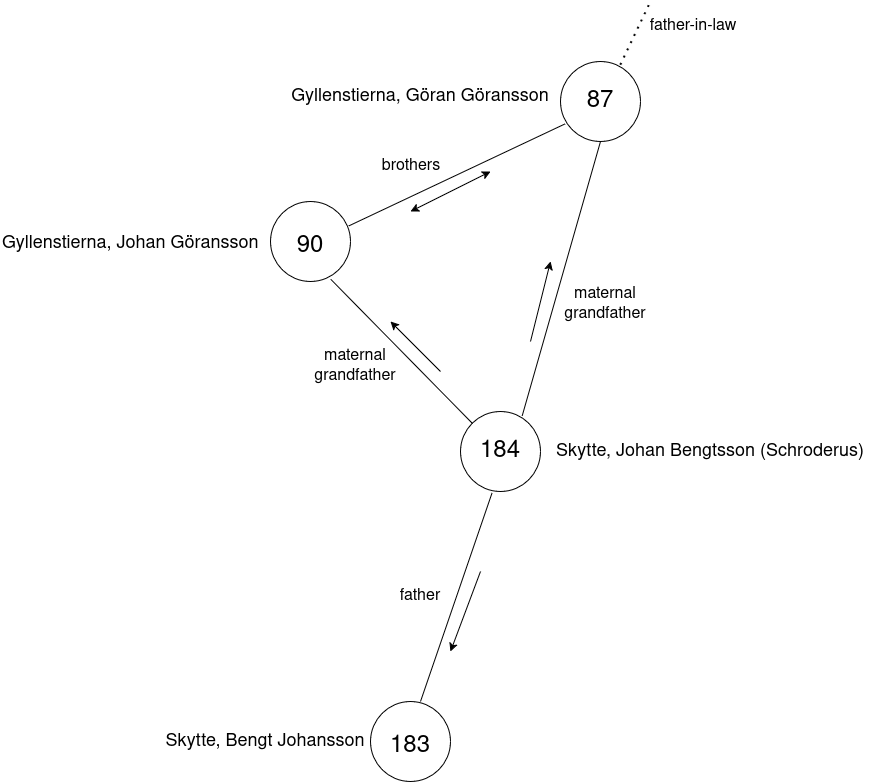
\includegraphics[scale=0.25]{example_network.drawio.png}
	\centering
	\caption{A sample from the graph} 
	\centering
\end{figure}
In this context the graph's nodes depict individual councillors with the input of name and id number. Correspondingly the edges represent the kinships between two nodes. For instance, in Figure 1 we can see that Johan Bengtsson (Schroderus) Skytte (id 184) is Bengt Johansson Skytte's (id 183) father and a maternal grandfather for Johan Göransson Gyllenstierna (id 90) and Göran Göransson Gyllenstierna (id 87). Johan Göransson and Göran Göransson are brothers, however, their father is not mentioned in the dataset. Göran Göransson also has further links in the network. \footfullcite{councillorsDS}

Calculating different statistics is a crucial part of the network analysis. One of the most important measures is the \textbf{node degree}. In all its simplicity node degree means the amount of edges connected to a specific node. For example, the degree of Johan Bengtsson (Schroderus) Skytte (id 184) is three or the degree of Bengt Johansson Skytte (id 183) is one. The \textbf{average degree} is the mean [keskiarvo] of all the node degrees of the specific graph. The \textbf{density} of the network is based on the node degrees. In very dense network almost every node is connected to each other, but a sparse graph has just a few edges in it.

Another important factor is whether the graph is \textbf{directed} or \textbf{undirected}. In directed graph the edges have directions, like in the communication networks a message has a sender and a receiver. The directions are marked with an arrow. In undirected graphs the edges are bidirectional (two way), for example, a relationship between two brothers can be understood as undirected. Directed graphs have more features and a more complex structures, for instance, the degrees of inbound and outbound edges can be counted separately. For sipmlicity, the graphs presented in this work are undirected.

\subsection{Implementation of the network analysis}
The data processing and analysis is conducted with a combination of Python programming language and Gephi software. Python is used for extracting the data from the councillors-dataset and formulating it in the right format: readable for Gephi. The actual network analysis, visualization and calculating statistics, is performed with Gephi. 

Python is a programming language popular amongst scientists. I selected Python due its simple syntax and ease in implementing small tasks like data processing. The language is understandable and widely used, which makes the work replicable. To be precise the script is written with Python 3.

As graphs are structures commonly used in programming, it would have been possible to conduct the actual network analysis using tools provided by Python, yet, Gephi software provides a visual user interface and more intuitive tools for the manipulation of the graph. Furthermore, the Gephi format makes the data and graph accessible also for non programmers.

Gephi is a software for network visualization and analysis. It contains tools for manipulating, filtering, clustering and visualizing the graph. It has built in appliances for fixing errors in data and calculating necessary statistics.\footcite{gephi} Gephi reads data from text format (comma separated values .csv) or Microsoft Excel tables (XLSX), and Gephi projects are saved as .gephi files. The processed graphs and data can be exported as images or tables.  

Nonetheless, Gephi does have some weaknesses. It is not always the most intuitive to use, and especially the visual configurations of the graph causes some issues. I have encountered difficulties with the node labels (the councilor's name next to the node). Sometimes the problems lies in the Gephi settings, but if the whole software crashes when trying to make the node labels visible, the problem lies within the software itself and should be solved when starting the program.\footnote{For Linux environments opening Gephi from command line with command "LIBGL\_ALWAYS\_SOFTWARE=1 ./gephi" can sometimes help.} 

Both of these tools are also open source and free to download. All scripts written for this work available on GitHub.\footnote{\url{https://github.com/Heidi-Suurkaulio/mastersthesis} TODO right link later}

Basically the steps of network analysis are : \begin{enumerate}
	\item Choosing the subject and data
	\item Pre processing the data for the network analysis
	\item Constructing the graph and finding possible issues and errors 
	\item Counting the statistics
	\item Deciding the layout (algorithm)
	\item Doing the interpretations
\end{enumerate}
However, the analysis is not that straightforward, sometimes the steps 2 and 3 must be repeated and re-repeated. Yet, on some circumstances the graph is not visualized or the statistics are not deemed important. These steps will be discussed in practice below.

\subsubsection{Test run}
%TODO fix councillor / councillor typo

To draft the structure of the graph and understand the nuances of the given data, a test run was carried out. The test run was done with a simple Python script, and no attention was paid to the temporal aspects of the network or the potential directions within the graph. The script and Gephi project used, and the visualization of the graph of the test run is available in GitHub in the TestRun folder\footnote{\url{https://github.com/Heidi-Suurkaulio/mastersthesis/tree/main/TestRun}}

The data processing was started by manually cleaning the data in LibreOffice Calc (equivalent to Microsoft Excel). The columns and rows containing information of the source material of the dataset and councillor's years active were removed. That made the structure of the data coherent and easier to manipulate with the Python script. The manually cleaned data is exported as .csv (comma separated values) file. The .csv file's header (the first line of the file) should be modified so that the column name "No." is changed to "Id" and "Family members in the council of the realm" is changed to "Family", the first one can cause an error if referenced in the Python code, the latter is inconveniently long.
%table 2

The script itself reads the data from the .csv file. The connections between the councillors are separated from the "Family" column, based on the knowledge that each connection is marked with the id number of another councillor. The connections are then formatted and printed to .csv file. The connections .csv file containing values for "Source" id of the source concillor, "Target" id of target councillor, "Type" standard "Undirected", "Id" id number for the connection, "Weight" standard 1.0. Another .csv file is formatted and printed with the information of councillors' names and id numbers.

\begin{table}[h]
	\caption{Example of the connections .csv file}
	\centering
	\begin{tabular}{cccccc}
		\hline
		1 &Source, &Target, &Type, &Id, &Weight \\
		\hline
		2 &231, &228, &Undirected, &0, &1.0 \\
		\hline
		3 &231, &230, &Undirected, &1, &1.0 \\
		\hline
	\end{tabular}
\end{table}
\begin{table}[h]
	\caption{Example of the councillors .csv file}
	\centering
	\begin{tabular}{ccc}	
		\hline
		1 &Id; &Label \\
		\hline
		2 &162; &Ingemar Petri \\
		\hline
		3 &231; &Tre Rosor, Ture Jönsson \\
		\hline
	\end{tabular}
\end{table}

These .csv files are readable for Gephi. The outcome was an undirected graph of the councillors' affiliation network that had accumulated during the 160 years. The graph consisted of 261 nodes (257 real + 4 "ghosts") and 372 edges (including self loops and "ghost" nodes). The test run revealed three problems within the graph: the emergence of the empty "ghost" nodes, parallel edges and thirdly self loops. 

The "ghost" nodes were excess nodes with no name and only an id number and one or two connections in the graph. They were due to the references to the data points removed from the original dataset, and therefore can be ignored. The ghosts are discussed further in the subsection \ref{sources}. However, the more essential problem were parallel edges and self loops.

The parallel edges occur because one relationship, such as father and son, is sometimes marked parallel in the dataset. For example, in the case of Göran Göransson Gyllenstierna (id 87) the relatives are "Maternal Grandfather 184, Brother 90, Father-in-law 3, ...", and the same relationship is found in his grandfather's Johan Bengtsson (Schroderus) Skytte's (id 184) links: "Son 183, Grandson through daughter 87". Yet, the connection to Göran Göransson's brother Johan Göransson Gyllenstierna (id 90) is not marked in the grandfathers links. This means that the node of Göran Göransson Gyllenstierna (id 87) has one excess link compared to his brother's node. The case is visualized in the Figure 2.

\begin{figure}[h]
	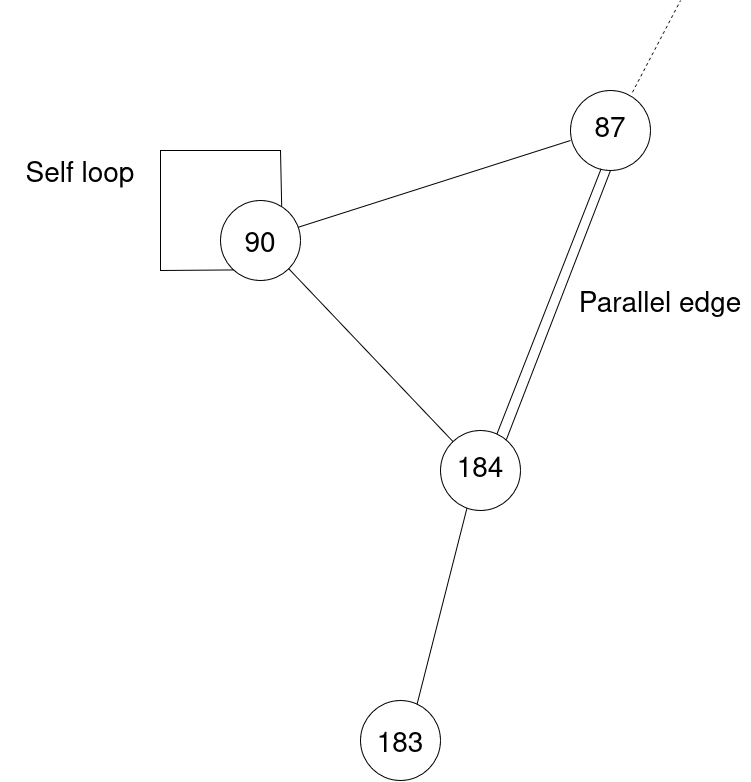
\includegraphics[scale=0.20]{double_link.drawio.png}
	\centering
	\caption{Visualisation of the parallel edge and self loop} 
	\centering
\end{figure}

These duplicate edges would cause bias to the calculation of the node degrees and any statistics based on them. A node degree is a sum of all the edges connected to one node, and if the relationships are inconsistently marked with one or two edges, the factually similar nodes would get different degrees. These inconsistent node degrees would accumulate when counting the average degrees an so forth. The problem of parallel edges is widely recognized in the field of network analysis, and therefore Gephi does have some builtin features for handling it.

While importing data to Gephi (on Import Spreadsheet) the strategy for merging the parallel edges can be chosen. One option is, for example, placing the sum or average of the parallel edges in the edge's degree, yet using only one connection to to represent the edge in the graph. In this context a more simple solution was chosen, with the option "Firs" Gephi will use only the first connection between two nodes ignoring any latter ones. This will reduce the amount of connections from 698 found in the connections.csv to only 372.

Self loops occur when one node has – for some reason or another – a connection to itself. Similarly to the parallel edges, they cause bias to the node degrees. In this graph a self loop can be found at least on the node with id 5 and id 90. In the case of id 5: Gustaf Axelsson Baner, his relatives are "Father 4, Father-in-law 217, Brother 9, Sons 5, 7, 8, 10, Sons-in-law 152 and 197", and similarly with id 90: Johan Göransson Gyllenstierna his family reads "Maternal Grandfather 184, Brother 90". These self loops are most likely caused by a typo in the dataset, because it is reasonable to assume that none is a son or brother to themselves.
 
Gephi does have a switch whether or not self loops are allowed in the graph, and it can automatically remove them based on the preference. The self loops are present in the test run graph alongside with the ghost nodes, yet those will be removed from the subsequent analysis. To highlight the ghosts they are colored cray, and the four nodes referred as an example here are colored red in the test run graph.

The last step in the preparation of the network analysis is the selection of the layout algorithm. For the test run an algorithm called Yifan Hu was used with default configurations except parameter theta set to 2.0. Then layout option "noOverlap" was chosen to separate possibly overlapping nodes, and some further manual placement of the nodes was done to make the graph more readable. The outcome was visually somewhat dense network in the middle and mostly unconnected isolated nodes around it. 

\subsection{Fitting modern model on historical timeperiod}
\begin{quote}
	Every model is an approximation.\\
	All models are wrong; some models are useful.\footcite[prefix]{statisticsfor}
\end{quote}

A graph is elementally a generalizing and simplifying model of complex social networks on the Swedish council of the Realm. Yet, when bulding any kinds of (computational) models, decisions between the complexity and abstraction must be made – in fact besides too simplifying models, too complex or overfitted ones are a problem on their own.\footcite{TODO} One of the most important question is what to include and and what to exclude. And, a more existential question is what we can model or even know about historical social networks. 

As I am working with pre-collected data, the choices have been made by the authors of the dataset Hakanen and Koskinen and by the scholars their work is leaning on. The data – and further the graph – is able to give a picture of the offically recorded family links within the council of the realm. However, it is not possible to know about the messy every day relationships, friendships, informal discussions, intentions, emotions or disputes these 257 men have had. It is important to understand the limitations of the data and model.

Generally, what comes to the study of early modern period, source material concerning women, lower social classes or marginalized groups are harder to find.\footcite{TODO} 
However, at least noble women are included in the contemporary lineage diagram as seen in figure \ref{queenlineage}. So maybe a network including noblewomen or the councilors patrons would be possible to build.

\begin{figure}
	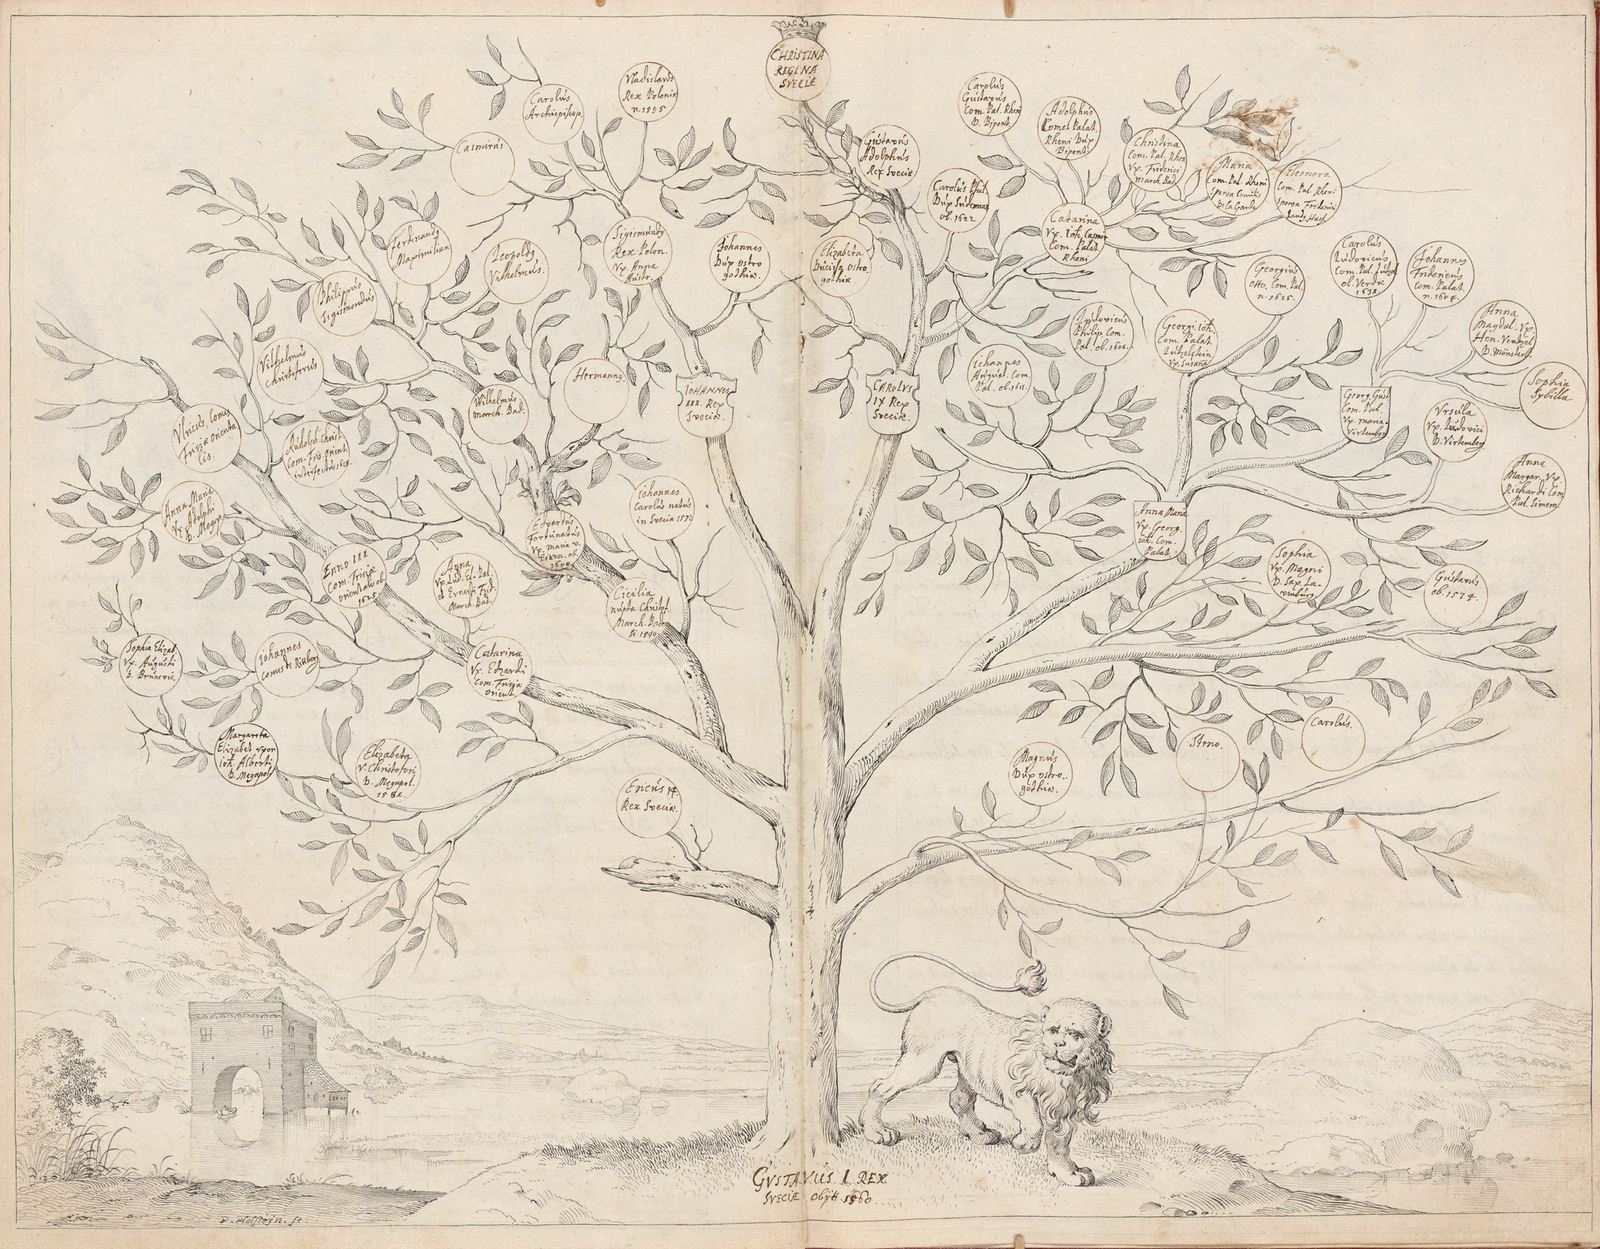
\includegraphics[width=\linewidth]{QueenChristinaLineage.png}
	\caption{Lineage of the house of Vasa from the \textit{Hortus Regius} or "Queen Christina's Genealogical Tree with Political Emblems".(\cite{hortusregius})} 
	\centering
	\label{queenlineage}
\end{figure}

It can be said with relative certainty that contemporaries in the early modern time didn't perceive their society as a network in the modern sense. And when studying ...
%TODO metonyme, biblical hierarchy, harmony
%TODO hopes and fears p. 21 - 22
%TODO personal agency p. 21

For instance \textit{Hortus Regius} can be used as an illustration of the ideals and understandings of the early modern nobility. The book was given to queen Christina by a diplomat Shering Rosenhane in circa 1645, and it consists of delicately illustrated political emblems\footnote{Instructions, virtues, metaphors} and noble family trees leading to queen Christina.\footcite{congresslibrary} 
%TODO explain the lineage diagram

		\newpage
		\section{Family Ties Between 1520 and 1680}
During the time period between 1520 and 1680 there were 257 men active in the Council of the Realm. As discussed earlier in subsection \ref{councilofrealm} the council consisted mostly of men with noble background. To quantify this: according to the dataset 236 of the 257 councillors (91.8\%) were part of the ancient nobility "uradel", and only approximately 5\% were of unknown or ignoble background, most of the time bishops or other clerics.  

\begin{table}
	\caption{Absolute amount in different ranks}
	\centering
	\begin{tabular}{cccccc}
		\hline
		Commoner & Ennobled & Estate unknown & Unknown & Ancient nobility & \\
		\hline
		5 & 8 & 7 & 1 & 236 & = 257 \\
		\hline
	\end{tabular}
	\caption{Proportional amount in different ranks}
	\centering
	\begin{tabular}{cccccc}
		\hline
	    Commoner & Ennobled & Estate unknown & Unknown & Ancient nobility & \\
	    \hline
	    1.9 & 3.1 & 2.7 & 0.3 & 91.8 & $\approx$ \% \\
	\end{tabular}
\end{table}

The kingdom of Sweden was ruled by nine monarchs: Gustavus Vasa (1523-1560), Eric XIV (1560-1568), Johan III (1568-1592), Sigismund (1592-1599), Charles IX (1599-1611), Gustavus Adolphus (1611-1632), Christina (1644-1654), Carl X Gustav (1654-1660) and Carles XI (1672-1697), and two regnants from 1632 to 1654 and from 1660 to 1672 during the time period. The amount of councillors appointed by each monarch\footnote{Calculated with a R script. To avoid the script dublicating the years that the monach changed, the beginning of each reign is adjusted, the actual year + 1. E. g. Eric XIV's reign is calculated 1561-1568, the actual being 1560-1668. This may cause slight inaccuracy.} or regnant varied from none to 56. Yet, 13 councillors were present before the reign of Gustavus Vasa.

The monarchs who appointed the most councillors were Gustavus Vasa (56) and queen Christina (45). The large number of councillors appointed by Gustavus Vasa may be explained by the sheer length of his reign. He ruled Sweden for 37 years, whereas all of the other monachs ruled less than 20 years. Also the religious Reformation was performed during his reign. The bishops and clerics that lost their position in the Council were replaced by noblement chosen by the king.\footcite[TODO]{pSuurvalta} As queen Christina ruled only for ten years, the exceptionally high number on her reign is interesting. Therefore, her reign will be discussed in greater detail in subsection \ref{christina}. 

However, the king who appointed no new councillors was the son of Johan III: Sigismund (1566-1632). He was both the king of Poland and Sweden forming a personal union between the two countries. Why king Sigismud did not appoint any new councillors? 

\begin{figure}
	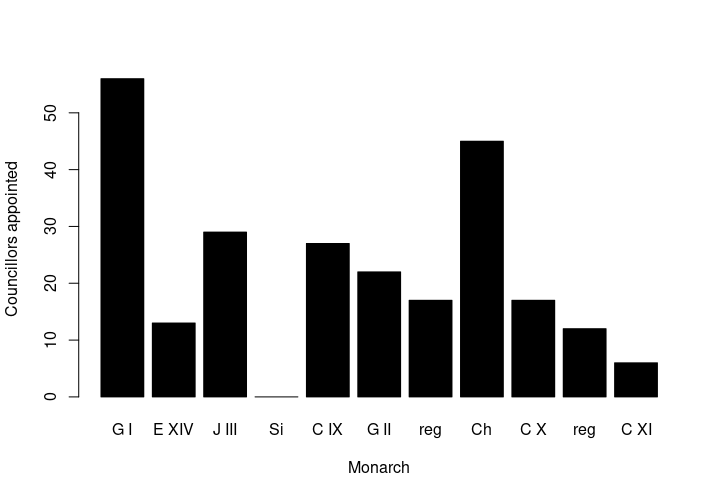
\includegraphics[scale=0.6]{councillorspermonarch.png}
	\centering
	\caption[Number of councillors appointed by each ruler between 1523-1680] {Number of councillors appointed by each monarch or regnant from 1523 to 1680. (\cite{councillorsDS}) Calculated and plotted with an R script: \url{https://github.com/Heidi-Suurkaulio/mastersthesis/blob/main/RScripts/councillors-1523-1680.R}.}
	\centering
\end{figure}

All of the councillors active between 1520 and 1680 are represented in a graph of 257 nodes and 362 edges, with self loops and parallel edges removed. The number of edges exceeds the number of nodes which means that theoretically all of the nodes could be linked to one another. Although, the edges are not distributed that way. Some of the nodes are linked to more than one other node, but some isolated nodes are indeed present. The average degree of the graph is 2.817 $\approx$ 2.8 meaning that councillors typically had 2 or 3 direct relations to another members of the Council.

The graph density is 0.011. In the mathematical definition the graph is sparse (scale from 0 to 1). However, interpretation in practical sense is not that straightforward. Having a completely dense social network, meaning that every node is directly linked to each other, is almost impossible. In this context it would mean, that each councillor is a direct relative through blood or marriage to each other, which would be weird to say at least. Further, taking the dimension of time into account, the mathematical interpretation would be even more nonsensical: how a nobleman appointed to the council in the 1670's could be directly linked to a bishop died in 1530's. 

The question wheither or not the councillors were higly linked to each other is more of a qualitative one. In the context of early modern institution, how we define a higly linked or even nepotistical institution? Probably the graph density has more explanatory value as a parameter to be compared between graphs collected from other contemporary communities.

Even so, the proportion of the nodes with at least one connection in the graph is $224/257 \approx 0.8715$ Which means that between 1520 and 1680 the probability of a councillor being related to someone else in the Council is $\approx$ 87\%. In that sense the councillors can be considered highly networked.

Another interesting finding are the nodes with the highest and lowest degree. Maybe the most eclectic and fascinating group is the isolated nodes. There are 33 isolated nodes meaning that 33 councillors did not have any family ties within the Council. Some of them are members of the nobility with family ties to councillors active prior the beginning year of the dataset, so the connections are excluded from this graph. These are for example: Ture Bengtsson Lilliesparre (127) or Nils Olofsson Vinge (242). Yet, some of the isolated nodes represent bishops and clerics like Magnus Sommar (186) or Ingemar Petri (162) present in the Council before the religious Reformation. 

Besides that, the isolated nodes also reveal something about the international relationships during the time period. For example a teacher from France Dionysius Beurraeus (12) or a Scottish baron Robert Douglas (58) can be found. Also the famous German born chancellor Conrad von Pyhy (168) is represented as an isolated node. During his stay in Sweden von Pyhy had a significant impact on the politics of Gustavus Vasa.\footcite[p. 81-83.]{pSuurvalta} This means that as a merited foreigner one could make their way up to the Swedish Council of the Realm.

On the contrary, the nodes with the highest degree ($\geq$ 5) are of councillors who are part of the old well established aristocratic families like De la Gardie, Oxentierna, Gyllenstierna, Bielke, Stenbock, Sparre and Ribbing. Also Finnish families of Horn and Kurck can be found.\footnote{TODO} That in itself ties to the previously known fact that the aristocratic families had a remarkable stance in the negotiations and politics of the Swedish kingdom.

To focus more on the temporal dimension of the graph, I decided to divide the dataset in half. As seen in Figure \ref{fig:peryear} the most intuitive point to do the division is between years 1600 and 1601. In year 1601 duke Charles had won the civil war against king Sigismund and he practically decimated the Council of the Realm while eliminating the noblemen loyal to the former king. However, by 1602 he had to appoint 15 new councillors in order to manage the growing number of tasks in diplomacy and administration.\footcite[TODO]{pSuurvalta} By coinsidence, year 1601 also divides the time range of the dataset in half. The first graph depicts the network prior to year 1600 and the latter one post year 1601, so both of these represent the family ties accumulated approximately for 80 years.

\subsection{Prior to Year 1600}
The graph depicts the family links within the Council during most of the 16th century. It consist of 111 nodes and 92 edges. In this case the number of edges subceeds the number of nodes meaning that at least some isolated nodes must be present. 

The average degree in this graph is 1.658 $\approx$ 1.7, meaning that typically councillors were directly related to one or two other members. The number is smaller than in the larger graph. However, it can be partly explained by the shorter time range, simply the family networks had not have enough time to accumulate. Thereafter, the closest comparison is the graph of councillors family ties post 1601, which will be discussed later.

The graph density is 0.015, allthough, comparing that to the larger graph is not that straightforward. The amount of nodes having at least one connection is $85/111 \approx 0.765$ meaning that the probability of councillors to be linked at least one other member is $\approx 77\%$. That is 10 percentage points smaller than in the larger graph. Even though this prior to year 1600 graph is not directly comparable with the larger graph, it indicates that the family links in the 16th century were more sparse.

The amount of isolated nodes is significant: 26–whereas in the larger graph it was 33. The fact that all of the bishops and clerics must be present in this graph partly explains this. Limiting the time range also breaks some of the existing links, so for example, Pontus De la Gardie seems to be without any connections in that graph, even though his descendands were remarkably woven into the networks of Swedish aristocracy. Taking these factors into account, still the relatively high number of isolated nodes may suggest the relatively high number of incomers and larger social mobility in general.

The nodes with highest degree ($\geq$ 4) were of the remarkable noble families such as Bielke and Stenbock, however the Bååt family is more apparent in this graph than in the larger one or any of the later ones (TODO check). Did the house lose its standing somehow, or did they blend with the other noble families?

\subsubsection{The Last Man Standing: Nils Gyllenstierna}
The latter half of the 16th century and espcially the turn of the 17th century was politically turbulent time in the kingdom of Sweden. The latter half of the 16th century being affected by the rivalry between the sons of Gustavus Vasa which culminated in the civil war during the 1590's. The battle between king Sigismund and duke Charles was won by duke Charles, who later directed his spite upon the Council of the Realm. Many of the councillors were executed or fled Sweden. Despite that the Council was almost fully devastated in 1601, one councillor was left behind: Nils Göransson Gyllenstierna (91).

Due to these circumstances, Nils Gyllenstierna had an exceptional political career. He was a nobleman born in 1526, and appointed to the Council (most likely) by Johan III in autumn 1560 at the age of 35. When he died of natural causes in 1601 at the age of 75, he had served a total of 41 years in the Council. Furthermore, he had been able to keep his position throughout all of the Gustavus Vasa's sons reigns.\footcite{councillorsDS} 

What led him to keep his position?

In fact, the last councillor to be executed in Sweden was Hogenskild Nilsson Bielke (16). He was born in 1538, and appointed to the Council by king Eric XIV in 1562 at the age of 24. He was inprisoned in Linköping in 1600 due to his incautious letters regarding duke Charles. He was executed in 1605 at the age of 67. All in all, he had served in the Council of the Realm for 36 years (being inactive for two years between 1590-1591).\footcites[p. 58.]{HakanenAKoskinen2017}{councillorsDS}

\subsection{Post Duke Charles' Revenge}
Practically, this graph begins from the year 1602 when duke Charles had to appoint 15 new councillors and the Council of the Realm was re-established. The graph consists of 146 nodes and 184 edges, now the number of edges exceeds the number of nodes. After 1601 (or 1602) the average degree of node is 2.251 $\approx$ 2.3, larger than the 1.7 prior to 1600. Also, visually the graph seems more dense. 

The number of isolated nodes is significantly lower: 16, compared to the 26 prior to 1600 or the 33 in the whole time period. Again it still must be remembered that limiting the time range cuts some family ties present in the dataset. Subsequently, the proportion of nodes with at least one edge is $130/146=0.890...$ ,thereby, the probability of councillor having at least one direct relation in the Council was now $\approx 89\%$. That is 12 precentage points greater than the 77\% in the 16th century, and two presentage points greater then the 87\% from the whole time period.

\begin{table}
	\caption[Number of edges needed for different densities of network]{Number of edges needed for different densities of network. The observed numbers are bolded}
	\label{edges}
	\begin{tabular}{cccc}
		\hline
		&& Amount of possible edges & \\
		\hline
		Density & 32 896 (all) & 6 105 (prior to 1600) & 10 585 (post 1601) \\
		\hline 
		0.011 & \textbf{361.9} & 67.2 & 116.4 \\
		\hline
		0.015 & 493.5 & \textbf{91.6} & 158.8 \\
		\hline
		0.0174 & 572.4 & 106.2 & \textbf{184.2}\\
		\hline
	\end{tabular}
\end{table}

Also the density of this graph is the largest: 0.017. In prior to 1600 it was 0.015 and from the whole time period 0.011. To make the densities comparable to some degree, the amount of edges needed for different densities is counted in Table \ref{edges}. Still, the scale of the larger graph makes it hard to compare with the other graphs, so, I will focus on the two smaller ones. The graph prior to 1600 would need $\approx 14$ more edges to have the density of 0.017, whereas in the graph post 1601 the difference between the density of 0.015 and 0.017 is $\approx 26$. This behaviour is explained in the subsection \ref{network}. So, even though the time scale is similar (80 years), the density and the absolute amount of edges is different. This means that it can be argumented that the post 1601 graph is more dense than the one prior to 1600. 

What the isolated nodes can tell us?

All in all, 17th century has been called in the previous literature "the century of the nobility", and the presented data seems to confirm the trend.\footnote{TODO} It seems that the family affiliations became more prominent in the Council of the Realm, and important in general, during the 17th century. Similarily, the amount of incomers decreased, which implies the slackening of social mobility.

\subsection{In the Court of Queen Christina}
\label{christina}
Queen Christina was the daughter of the king Gustavus Adolphus and queen consort Maria Eleonora of Brandenburg (1599-1655). She inherited the throne at the age of 6, after her fathers sudden death in the battlefield in November 1632. Before she was declared an adult at the age of 18 in 1644, the kingdom was ruled by a regnant.\footnote{TODO source} The reign and personal life of queen Christina are fascinating chapters in the Swedish history.\footnote{For more information see e.g. Peter Englund \textit{Silvermasken: en kort biografi över drottning Kristina} finnish version \textit{Kuningatar Kristiina}, or Marie-Louise Rodén \textit{Drottning Christina: en biografi}.}

Due that Christina's father was frequently away from Sweden and the long period of the interregnum, the authority of the Council of the Realm had grown remarkably when Christina was enthroned. Contrary to the previous monarchs, she was forced to go for the Council to get councel, yet, the situation did not stay that way for long. In the words of Hakanen and Koskinen: 

\begin{quote}
	Christina played the high nobility at their own social network game rather than enter into open warfare with them. That is, she quickly created a large group of loyal supporters around her $\dots$
\end{quote}

Furthermore, she appointed many new councillors to dilute the power of the original Council. By the year 1654 she had appointed 45 new councillors.\footcite[p. 64. ]{HakanenAKoskinen2017}

The network of councillors appointed by queen Christina is displayed in Figure \ref{queenChristinaCouncillors}. As queen Christina's reign lasted for only ten years the graph is not comparable to the other larger graphs, despite that, it is interesting in its own right. The graph consist of 45 councillors, all of them which must have been close to queen Christina in one way or another.

\begin{figure}	
	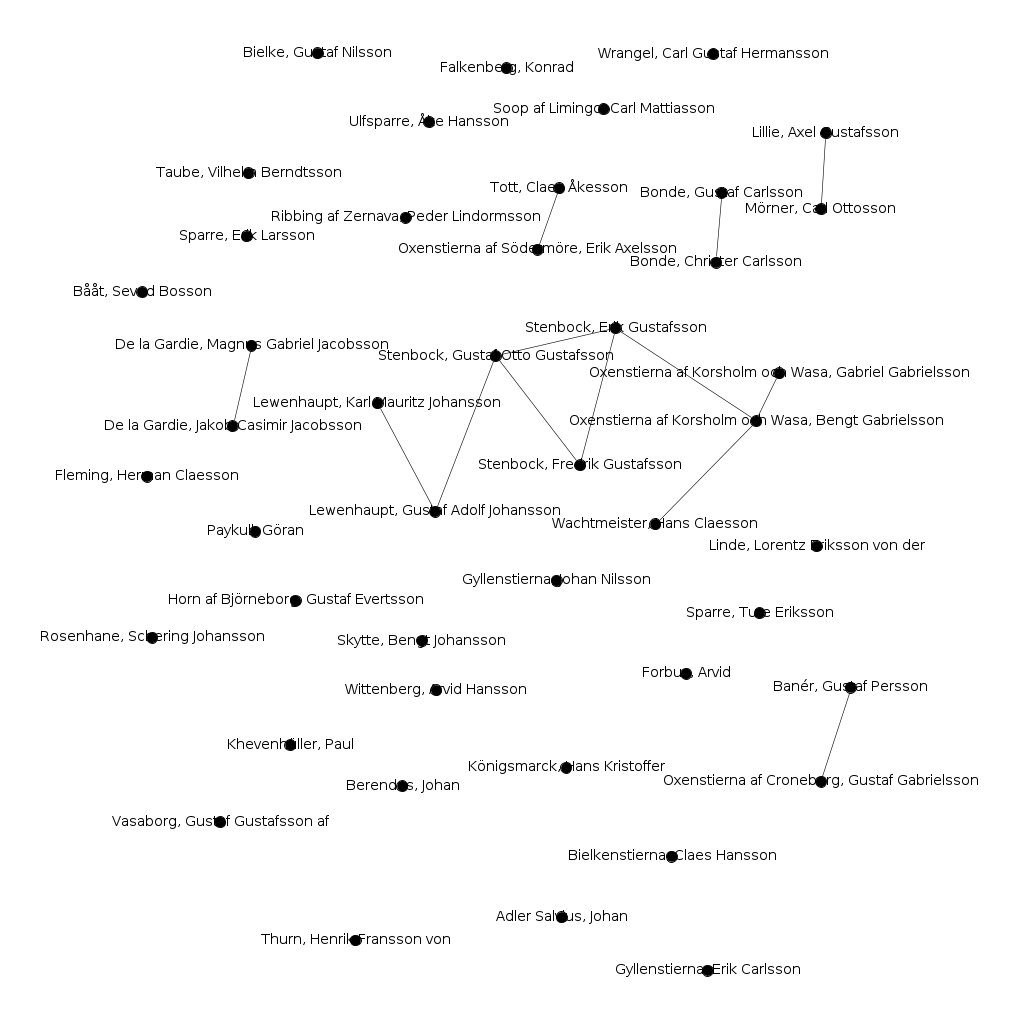
\includegraphics[width=\linewidth]{councillors_1644-1654.png}
	\caption[Councillors appointed by queen Christina]{A graph of councillors appointed by queen Christina between 1644 and 1654.(\cite{councillorsDS})}
	\label{queenChristinaCouncillors}
	\centering
\end{figure}

Overall, the network seems sparse, but, an interestingly clustered pattern can be found in the middle of the network. Eight councillors: Karl Mauritz Johansson Lewenhaupt (125), Gustaf Adolf Johansson Lewenhaupt (126), Gustaf Otto Gustafsson Stenbock (207), Fredrik Gustafssonare Stenbock (204), Erik Gustafssonall Stenbock (202), Bengt Gabrielsson Oxenstierna af Korsholm och Wasa (148), Gabriel Gabrielsson Oxenstierna af Korsholm och Wasa (154) and Hans Claesson Wachtmeister (240) are all related to each other direclty or indirectly. 

This tightly woven network seems to concentrate around the two brothers Gustaf Otto Gustafsson Stenbock and Erik Gustafssonall Stenbock. Due that they presumably had a significant position in the political life. What led them having this position?

Some other interesting individuals can be also found in the graph. Christina appointed his paternal half brother Gustaf Gustafsson af Vasaborg (241)–Gustavus Adolphus' illegitimate son–to the Council on 5th of September 1646. Also the diplomat and nobleman Schering Johansson Rosenhane (177) who gave queen Christina the Hortus Regius -manuscript was appointed to the Council by Christina on 30th of September 1650.\footcite{councillorsDS} This may mean that family ties–even illegitimate–were of high value, but also mutual relationships had their place in the political sphere of early modern Sweden.

		\newpage
		\section{Conclusion}
Network analysis can reveal new patterns on the family networks of the Swedish councillors of the Realm, but in this case, it mostly seems to support the already known. The graphs depicting the councillors' family ties in the early modern period are highly linked for the most part. This, in accordance with the previous research, indicates that an individual's place in the society was determined by the family background. Yet, the density of the networks–depicting the importance of the family relations–changes with time. The graph of the 16th century is more sparse than the graph of the 17th century.

Probably one of the most telling part of the graphs were the isolated nodes or lack of thereof. In the graph depicting the 16th century, the isolated nodes were somewhat common, but the amount decreased in the 17th century graph. In some cases the nodes were of incomers to the Swedish political life, and therefore indicating social mobility. The councillors represented by these nodes usually led interesting life stories.

When it comes to the question of noble houses, the graphs did not form visually separate subgraphs or components, which would indicate individual families or houses. Instead the well established and famous noble lines such as Gyllenstierna, De la Gardie and Sparre were present in the nodes with the most connections. In that case it seems that the family networks were connected to each other, and most prominent houses were integrally intervowen into the network of the councillors of the Realm.

Collecting and creating network data manually from scratch is a daunting and time consuming task. To make process of building the graphs from already existing data easier, I coded a small Python script to do the manual, error prone and dull work for me. Altogether, automatizing the process of extracting historical data is not that straightforward.

\begin{quote}
	Here is a truth: nobody wants to run your program. What they want is to get their work done, or play their game, or send their email\ldots The truth is that good code is invisible. It simply allows things to flow smoothly. Bad code is memorable. It interferes, makes people frustrated and angry.\footcite[prefix p. XVI]{python}
\end{quote}

Automatically processing data that is not designed and collected to be automatically processed is hard. Scripts do not have an understanding of context. If the dataset or file names contain minor characters, such as dots or spaces, the script may crash. These detrimental small characters have to be manually replaced from the dataset or to be excluded from the processed data. Also the slighest changes in the spelling is able to corrupt the whole model.

For instance, working on a similar task for the \textit{Shared Past, Different Interpretations} -project, I came across two different spellings of the same name in the dataset. This caused the script to create two nodes, of the one and same person to the graph. To make matters worse, the person was a highly central figure on the network, and the conflicting nodes discretely broke the whole model. With the help of alert colleaque, and by a lucky coinsidence, the error was spotted in time. Had that not happened, the graph would have remained inherently inaccurate. Usually it helps, if the programmer–or the working group–has at least conceptual understanding of the data. 

An important observation concerning the actual network analysis is which statistics are usable in the context of historical social networks. For example, the graph density should tell us how interwoven the network was. Instead, as the number of possible nodes increases so rapidly with the size of the network, the density of two networks, with even a little difference in size, is almost impossible to compare. Furthermore, the mathematical definition of dense network would be odd in the context of larger social networks. On the other hand, the far simpler parameters, such as node degree or the ratio of isolated nodes from all nodes, are way more depicting. 

While doing this work I made some simplifications on the data processing and model building. For instance, the calculated and reported numbers of edges are in fact the lower limit of the probable numbers. While limiting the time range of the graphs, some existing family links are excluded from the calculation, and, furthermore, some links were already excluded from the original dataset. This means that the actual networks were most likely slightly more linked. This deviation or uncertainty could be further quantified with the methods of Bayesian statistics.
 
As computational network analysis seems to be a working method in the study of early modern history, it could be implemented in the study of wider social groups. Reconstructing social networks with noble women or the clients of the noblemen could be a doable task in the future.

%TODO  parallel edges, ghosts
	\end{onehalfspace}
\newpage
\printbibliography[heading=bibintoc,type=misc,title={References}]
\printbibliography[heading=subbibintoc,filter=literature,title={Literature}]
\printbibliography[heading=subbibintoc,type=online,title={Online}]
\printbibliography[heading=subbibintoc,type=manual,title={Documentation}]
\newpage
\appendix
\section{the Script to End All Scripts}
\label{script}
\begin{small}
\begin{verbatim}
__author__ = "Heidi Suurkaulio"
__dependencies__ = ["sys", "pandas", "csv", "re"]
__version__ = "1.0"
__date__ = "01-05-2025"
__project__ = "https://github.com/Heidi-Suurkaulio/mastersthesis"
__maintainer__ = "Heidi Suurkaulio"
__email__ = "heidisuur@gmail.com"

import sys
import pandas as pd
from csv import writer
import re

# testing that the filename is present
if len(sys.argv) < 2:
    print("Error: file name must be given in format .csv")
    sys.exit()

# reading the data
dataset_name = sys.argv[1]
dataset = pd.read_csv(dataset_name ,sep=";", index_col="Id")
dataset["Connections"] = None

# make sure the years of appointment are numeric type
dataset.update(pd.to_numeric(dataset['Appointed']))

# if start and end year or interval is given, limits the dataset on given parameters
if len(sys.argv) == 4:
    match sys.argv[2]:
        case "prior":
            # the year of appointment is the same or smaller than given
            end_year = int(sys.argv[3])
            dataset = dataset.loc[dataset['Appointed'] <= end_year]
        case "post":
            # the year of appointment is the same or greater than given
            start_year = int(sys.argv[3])
            dataset = dataset.loc[dataset['Appointed'] >= start_year]
        case default:
            # the year of appointment is greater than the first year given
            # the year of appointment is smaller than the last year given
            start_year = int(sys.argv[2])
            dataset = dataset.loc[dataset['Appointed'] >= start_year]
            end_year = int(sys.argv[3])
            dataset = dataset.loc[dataset['Appointed'] <= end_year]       
\end{verbatim}
\pagebreak
\begin{verbatim}
# save the connections to the dataset
for index, ent in dataset.iterrows():
    st = ent.Family
    if isinstance(st, str):
        cons = re.findall(r'\b\d+\b', st)
        cons = list(map(int, cons)) # convert to integer
        dataset.at[index, "Connections"] = cons

# find current indexes
current_ids = dataset.index

# make a list of connections
printable = []
printable.append(['Source', 'Target', 'Type', 'Id', 'Weight'])
i = 0
for index, entr in dataset.iterrows():
    if isinstance(entr.Connections, list) and len(entr.Connections) > 0:
    for o in entr.Connections:
        if o in current_ids: # check if the id mentioned in connection is in dataset
            printable.append([index, o, "Undirected", i ,"1.0"])
            i = i + 1

# print all
dataset.to_csv("councillors.csv", columns=["Name"], sep=";", header=["Label"])

with open("connections.csv", "w", newline='') as csvfile:
    wr = writer(csvfile)
    wr.writerows(printable)
\end{verbatim}
\end{small}
\section{Graph 1520-1680}
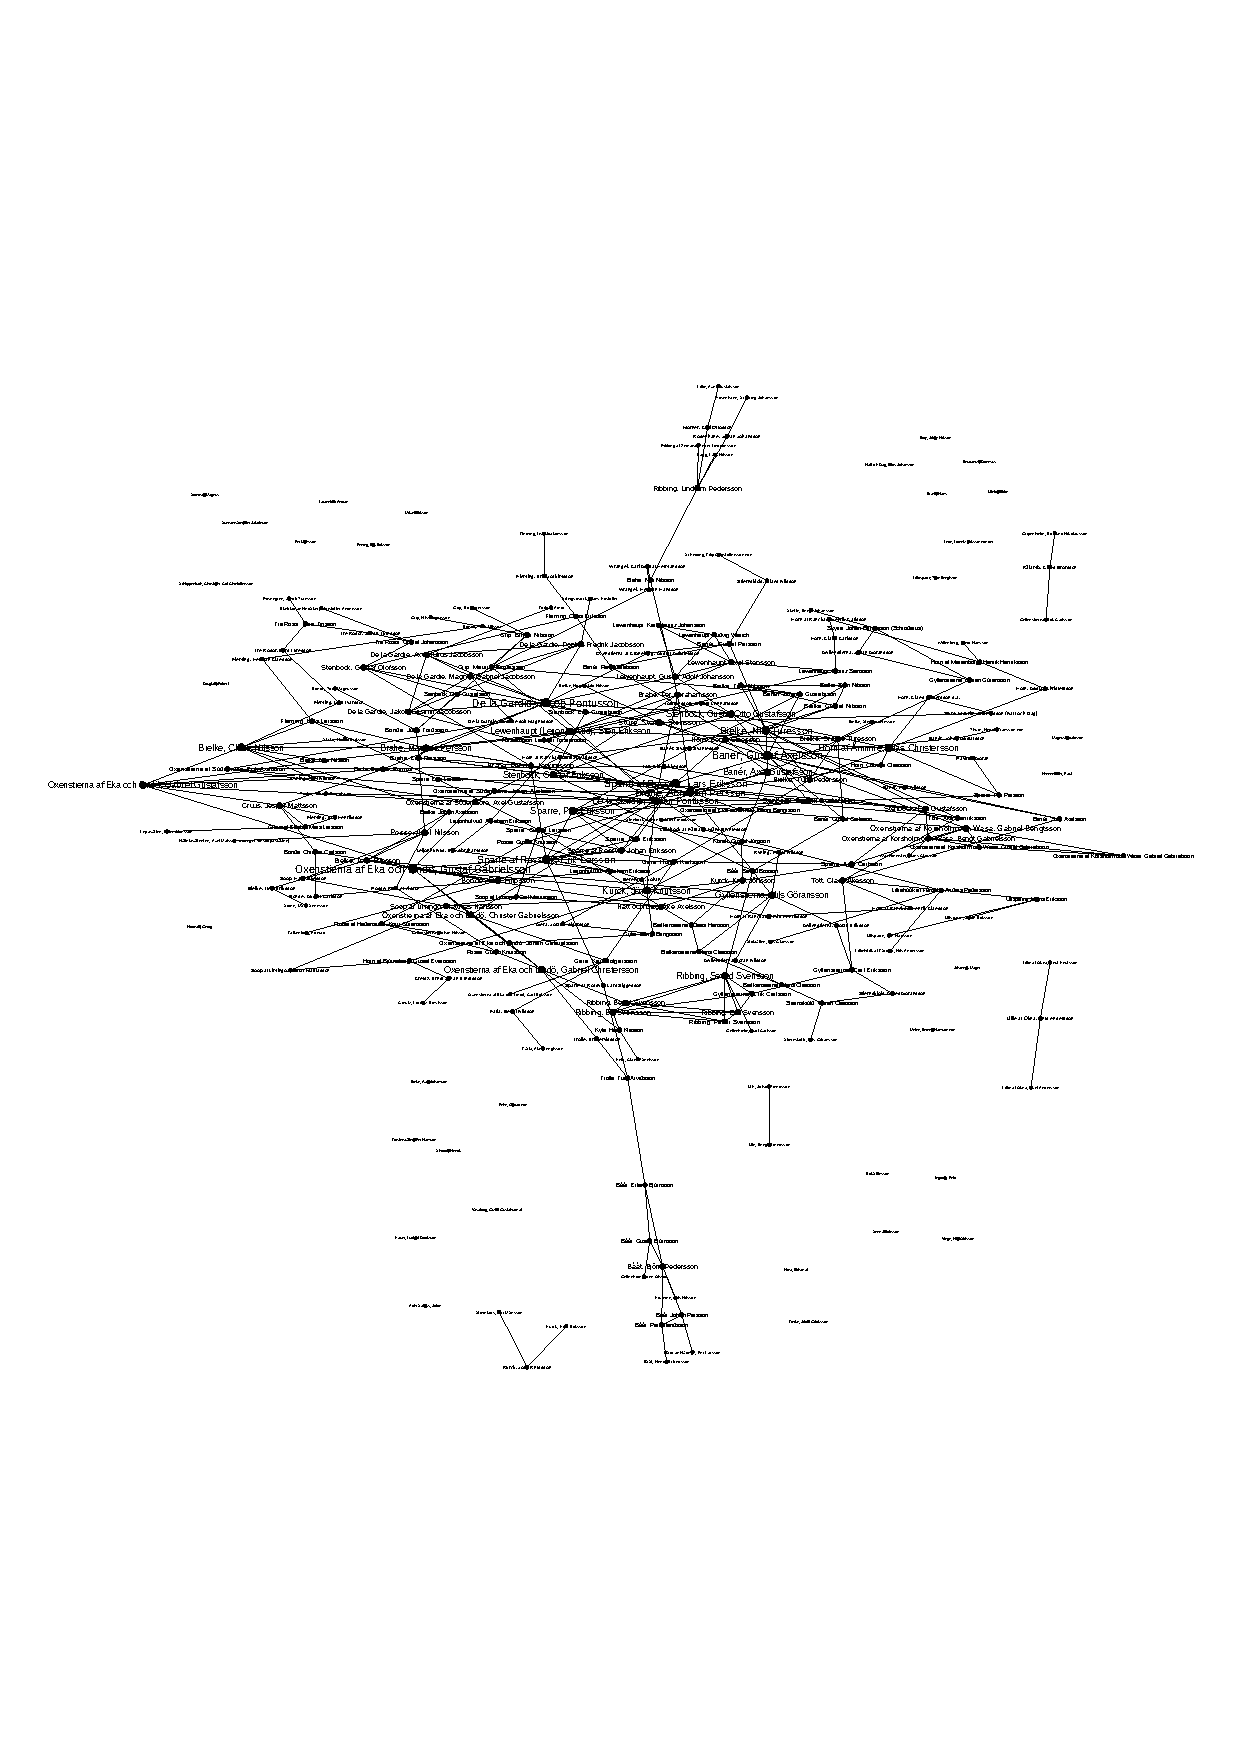
\includegraphics[width=\linewidth]{councillors_of_the_realm_1520-1680.pdf}
Higher resolution available in: \url{https://github.com/Heidi-Suurkaulio/mastersthesis/tree/main/GephiProjects}
\section{Graph Prior 1600}
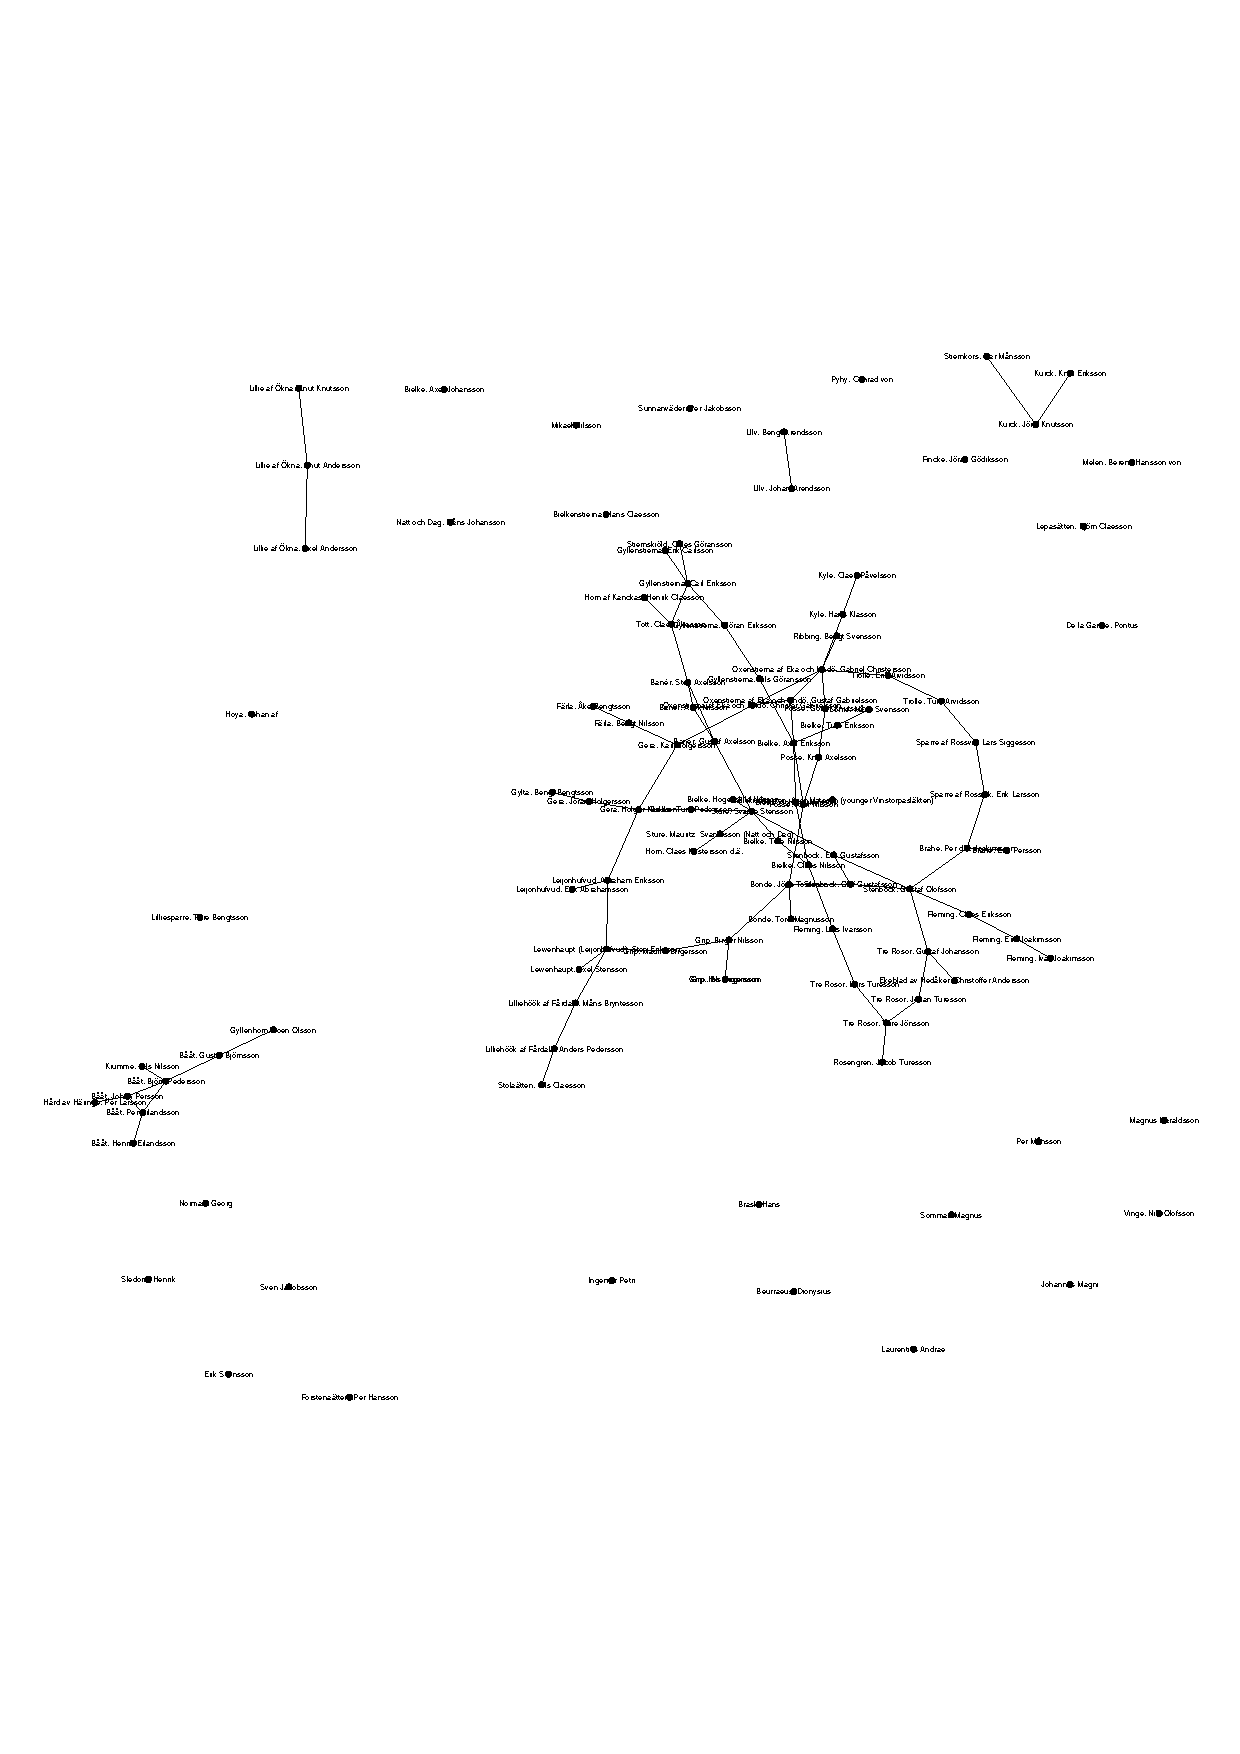
\includegraphics[width=\linewidth]{councillors_prior1600.pdf}
Higher resolution available in: \url{URL}
\section{Graph Post 1601}
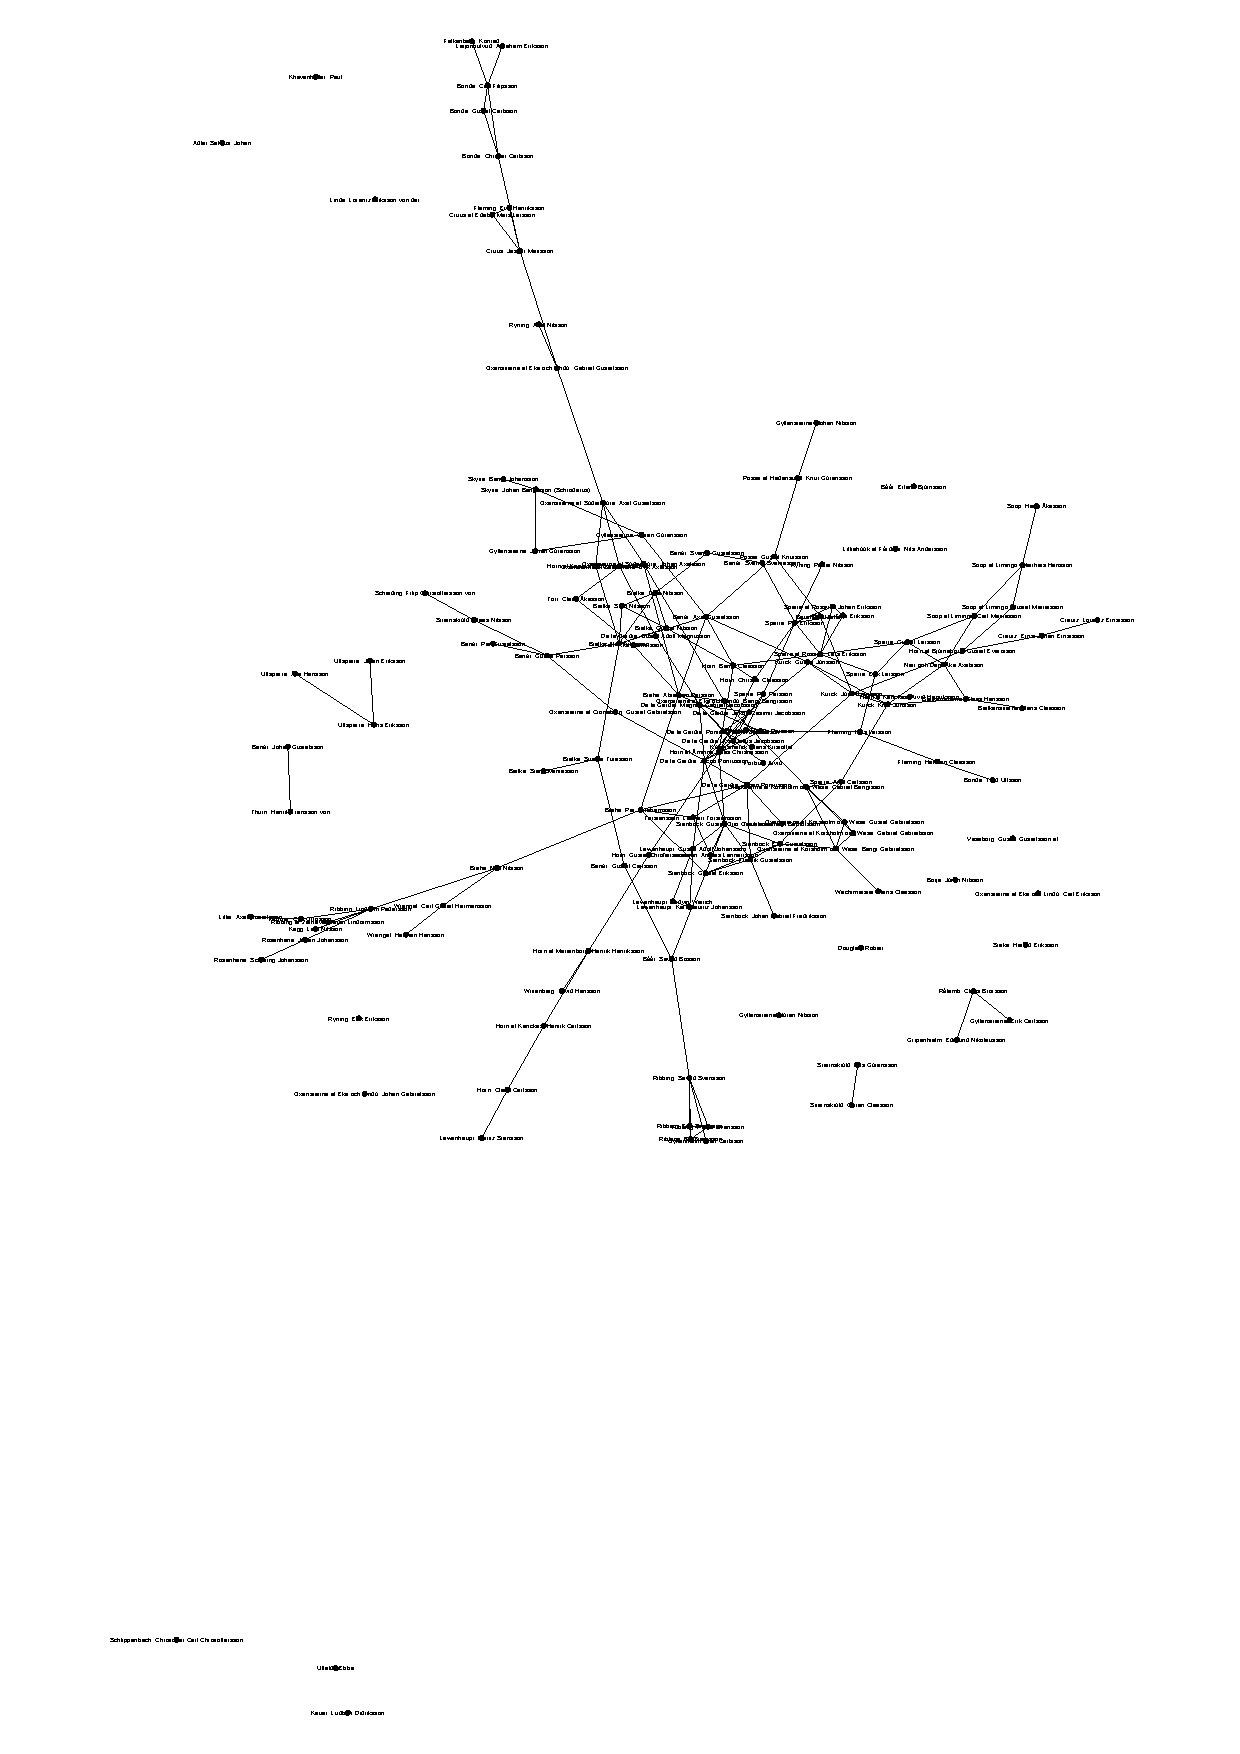
\includegraphics[width=\linewidth]{councillors_post1601.pdf}
Higher resolution available in: \url{https://github.com/Heidi-Suurkaulio/mastersthesis/tree/main/GephiProjects}
\end{document}